\documentclass{beamer}
\usepackage{coloremoji}
\usepackage{graphicx,url}
\usepackage[brazil]{babel}
\usepackage{minted}
\usepackage{inputenc}
\usepackage{pgf,tikz}
\usepackage{adjustbox}
\usepackage{mathrsfs}
\usepackage{xcolor}
\usepackage{soul}
%\usepackage{listings}
\usetikzlibrary{calc}
\usetikzlibrary{arrows}
\batchmode
\usepackage{amsmath,amssymb,enumerate,epsfig,bbm,calc,color,ifthen,capt-of}
\usetheme{Berlin}
\definecolor{mygray}{gray}{0.9}
%-------------------------Titulo/Autores/Orientador------------------------------------------------
\title[Monash Competitive Programming Club]{Intro to Competitive Programming}
\subtitle {MCPC Workshop}
\date{}
\author[Eggeek (Shizhe Zhao)]{
}

\pgfdeclareimage[height=1.0cm]{icpc-logo}{../icpc.pdf}
\logo{\pgfuseimage{icpc-logo}\hspace*{0.5cm}}

\AtBeginSection[]
{
  \begin{frame}<beamer>
    \frametitle{Outline}
    \tableofcontents[currentsection]
  \end{frame}
}
%\setbeamercovered{transparent}
%\beamerdefaultoverlayspecification{<+->}
% -----------------------------------------------------------------------------
\begin{document}
% -----------------------------------------------------------------------------

%---Summary---------------------------------------------------------
\frame{\titlepage}
\section[]{}
% \begin{frame}{Summary}
%   \tableofcontents
% \end{frame}

\section{What}
\begin{frame}{What's the Competitive Programming}
Briefly speaking, it is to solve programming problems:
\begin{itemize}
  \item<2-> Fast
  \item<3-> Correctly
  \item<4-> Elegantly
\end{itemize}
\end{frame}

\section{Sugar}
\begin{frame}{Get lowest bit}
\begin{columns}
  \begin{column}{0.5\columnwidth}
  \onslide<1-> The common way:
  \inputminted[linenos=true, fontsize=\small, bgcolor=mygray, ]{python}{./src/lowb0.py}
  \end{column}
  \begin{column}{0.5\columnwidth}
    \onslide<2-> In competitive programming:
    \inputminted[linenos=true, fontsize=\small, bgcolor=mygray, ]{python}{./src/lowb.py}
  \end{column}
\end{columns}
\end{frame}

\begin{frame}{Prime Sieve}
\onslide<1-> The straightforward way:
\inputminted[linenos=true, fontsize=\scriptsize, bgcolor=mygray, ]{python}{./src/prime0.py}
  \onslide<2-> \small $2+3+2+5+\ldots \approx O(\frac{n^2}{log n})$ (\url{https://oeis.org/A088821})
\end{frame}

\begin{frame}{Prime Sieve}
\onslide<1-> More efficient way:
\inputminted[linenos=true, fontsize=\scriptsize, bgcolor=mygray, ]{python}{./src/prime1.py}
  \onslide<2-> \small $\frac{n}{2} + \frac{n}{3} + \ldots + 1 \approx O(nlogn)$ (Harmonic sequence)
\end{frame}

\begin{frame}{Prime Sieve}
  \onslide<1-> In competitive programming:
  \begin{itemize}
    \item<2-> \small Each number only be sieved by it's minimum prime factor once.
    \item<3-> \small It's linear!
  \end{itemize}
  \inputminted[linenos=true, fontsize=\scriptsize, bgcolor=mygray, ]{python}{./src/prime2.py}
\end{frame}

\begin{frame}{$A+B$}
\begin{columns}
  \begin{column}{0.48\columnwidth}
  \onslide<1-> The common way:
  \inputminted[linenos=true, fontsize=\scriptsize, bgcolor=mygray, ]{python}{./src/plus0.py}
  \end{column}
  \begin{column}{0.48\columnwidth}
    \onslide<2-> In competitive programming:
    \inputminted[linenos=true, fontsize=\scriptsize, bgcolor=mygray, ]{python}{./src/plus1.py}
  \end{column}
\end{columns}

\begin{columns}
  \begin{column}{0.6\columnwidth}
  \onslide<3->
    \begin{figure}
      \centering
      
\includegraphics[width=.35\textwidth]{pic/rage.jpeg}
    \end{figure}
  \end{column}
  \begin{column}{0.4\columnwidth}
    \onslide<3-> \st{Creative!}
  \end{column}
\end{columns}
\end{frame}

\section{Why}
\begin{frame}{Why}
  \centering
  \huge{Why do we do Competitive Programming?}
\end{frame}

\begin{frame}{An Imagination}
\begin{itemize}
  \item<1-> You want to be a top-class programmer 😎.
  \item<2-> There are lots of choices: 😱
    \begin{itemize}
      \item<3-> Web full stack, Mobile dev,
      Database, Big data, Machine learning \ldots
    \end{itemize}
  \item<4-> Oh, you choosed \textit{Web full stack} 😃.
  \item<5-> What is going to happend next...? 😯
\end{itemize}
\end{frame}

\begin{frame}{An Imagination}
You...
\begin{itemize}
  \item<2-> may find a nice online resource. 😀
  \item<3-> follow the instructions. 😀
  \item<4-> may need hours to set up environment. 🕖🕗🕘
  \item<5-> finally finish your first demo before sleep. 😐
\end{itemize}
\onslide<6-> but what can you still remember in the next day, or next week? 😳
\end{frame}

\begin{frame}{Reflection}
\begin{itemize}
  \item<2-> We are distracted by those \textit{working skill}s,
  \item<3-> It's not too late to pick up these in future career ($\ge 30$ years),
  \item<4-> but we only have two to four years in university.
  \item<5-> Looking for a more efficient way?
\end{itemize}
\end{frame}

\begin{frame}{Why}
\onslide<1-> Compeititve programming is most efficient way to:
\begin{itemize}
  \item<2-> improve coding skill
  \item<3-> improve problem solving skill
  \item<4-> develop insight in computer science
\end{itemize}
\onslide<5-> There is another story...
\end{frame}

\begin{frame}{Another Story}
\begin{itemize}
  \item<1-> You want to be a top-class programmer.😎
  \item<2-> Someone suggests you to do Competitive Programming.😉
  \item<3-> What is going to happend next...? 😯
\end{itemize}
\end{frame}

\begin{frame}{Another Story}
\begin{minipage}{.75\textwidth}
  \begin{adjustbox}{max totalsize={1.\textwidth}{1.\textheight}, left}
  \centering
  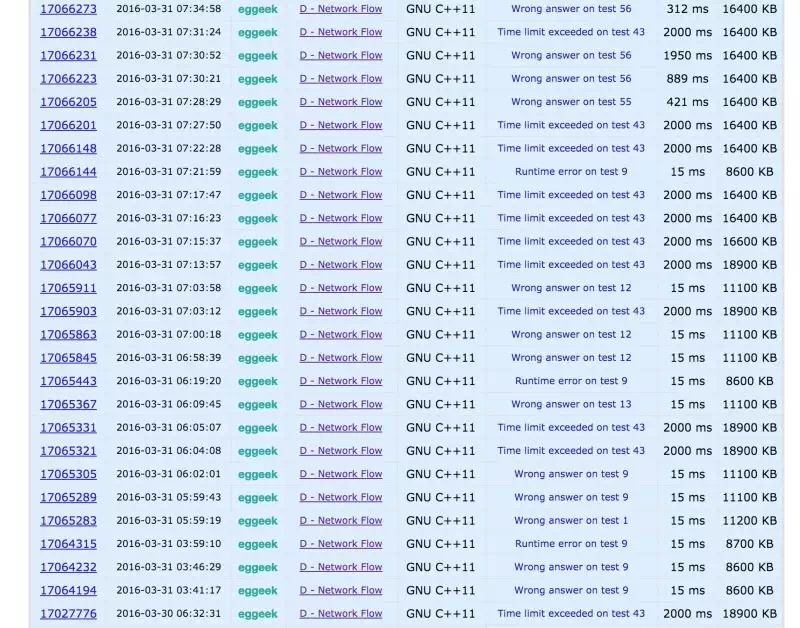
\includegraphics[width=\textwidth]{pic/sub0.jpg}
  \end{adjustbox}
\end{minipage}%
\begin{minipage}{.25\textwidth}
  Practice!
\end{minipage}
\end{frame}

\begin{frame}{Another Story}
\begin{minipage}{.75\textwidth}
  \begin{adjustbox}{max totalsize={1.\textwidth}{1.\textheight}, left}
  \centering
  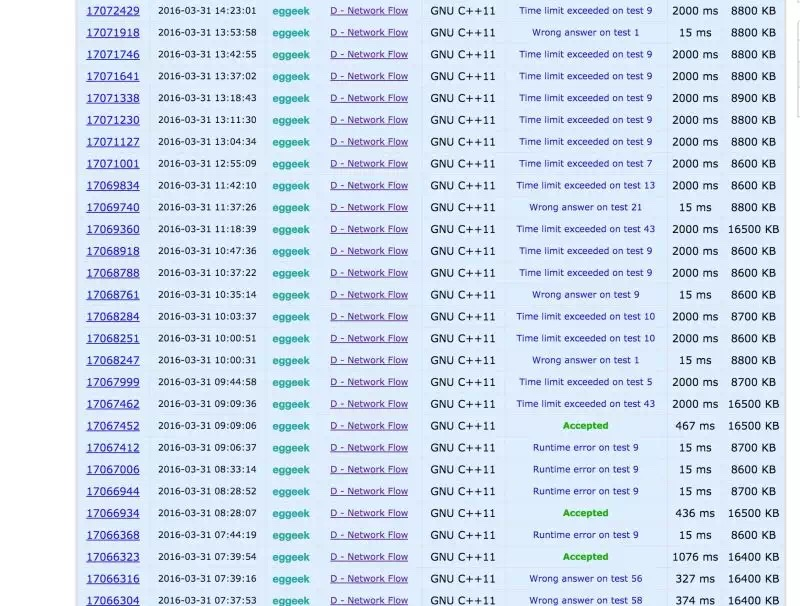
\includegraphics[width=\textwidth]{pic/sub1.jpg}
  \end{adjustbox}
\end{minipage}%
\begin{minipage}{.25\textwidth}
  Keep practicing!
\end{minipage}
\end{frame}

\begin{frame}{Another Story}
  \begin{figure}
  \centering
  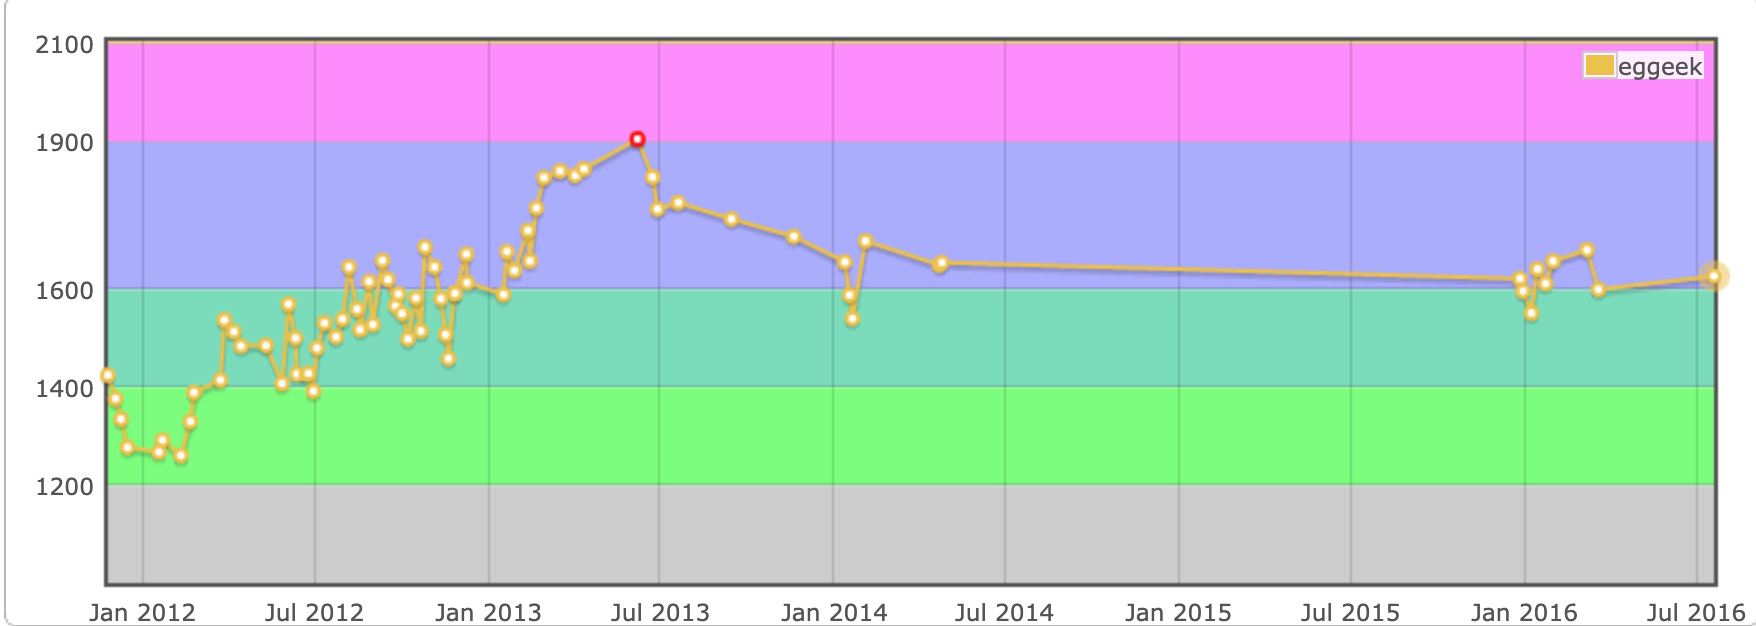
\includegraphics[width=\textwidth]{pic/rating.png}
  \end{figure}
  Win and lose...
\end{frame}

\begin{frame}{Another Story}
  \begin{figure}
  \centering
  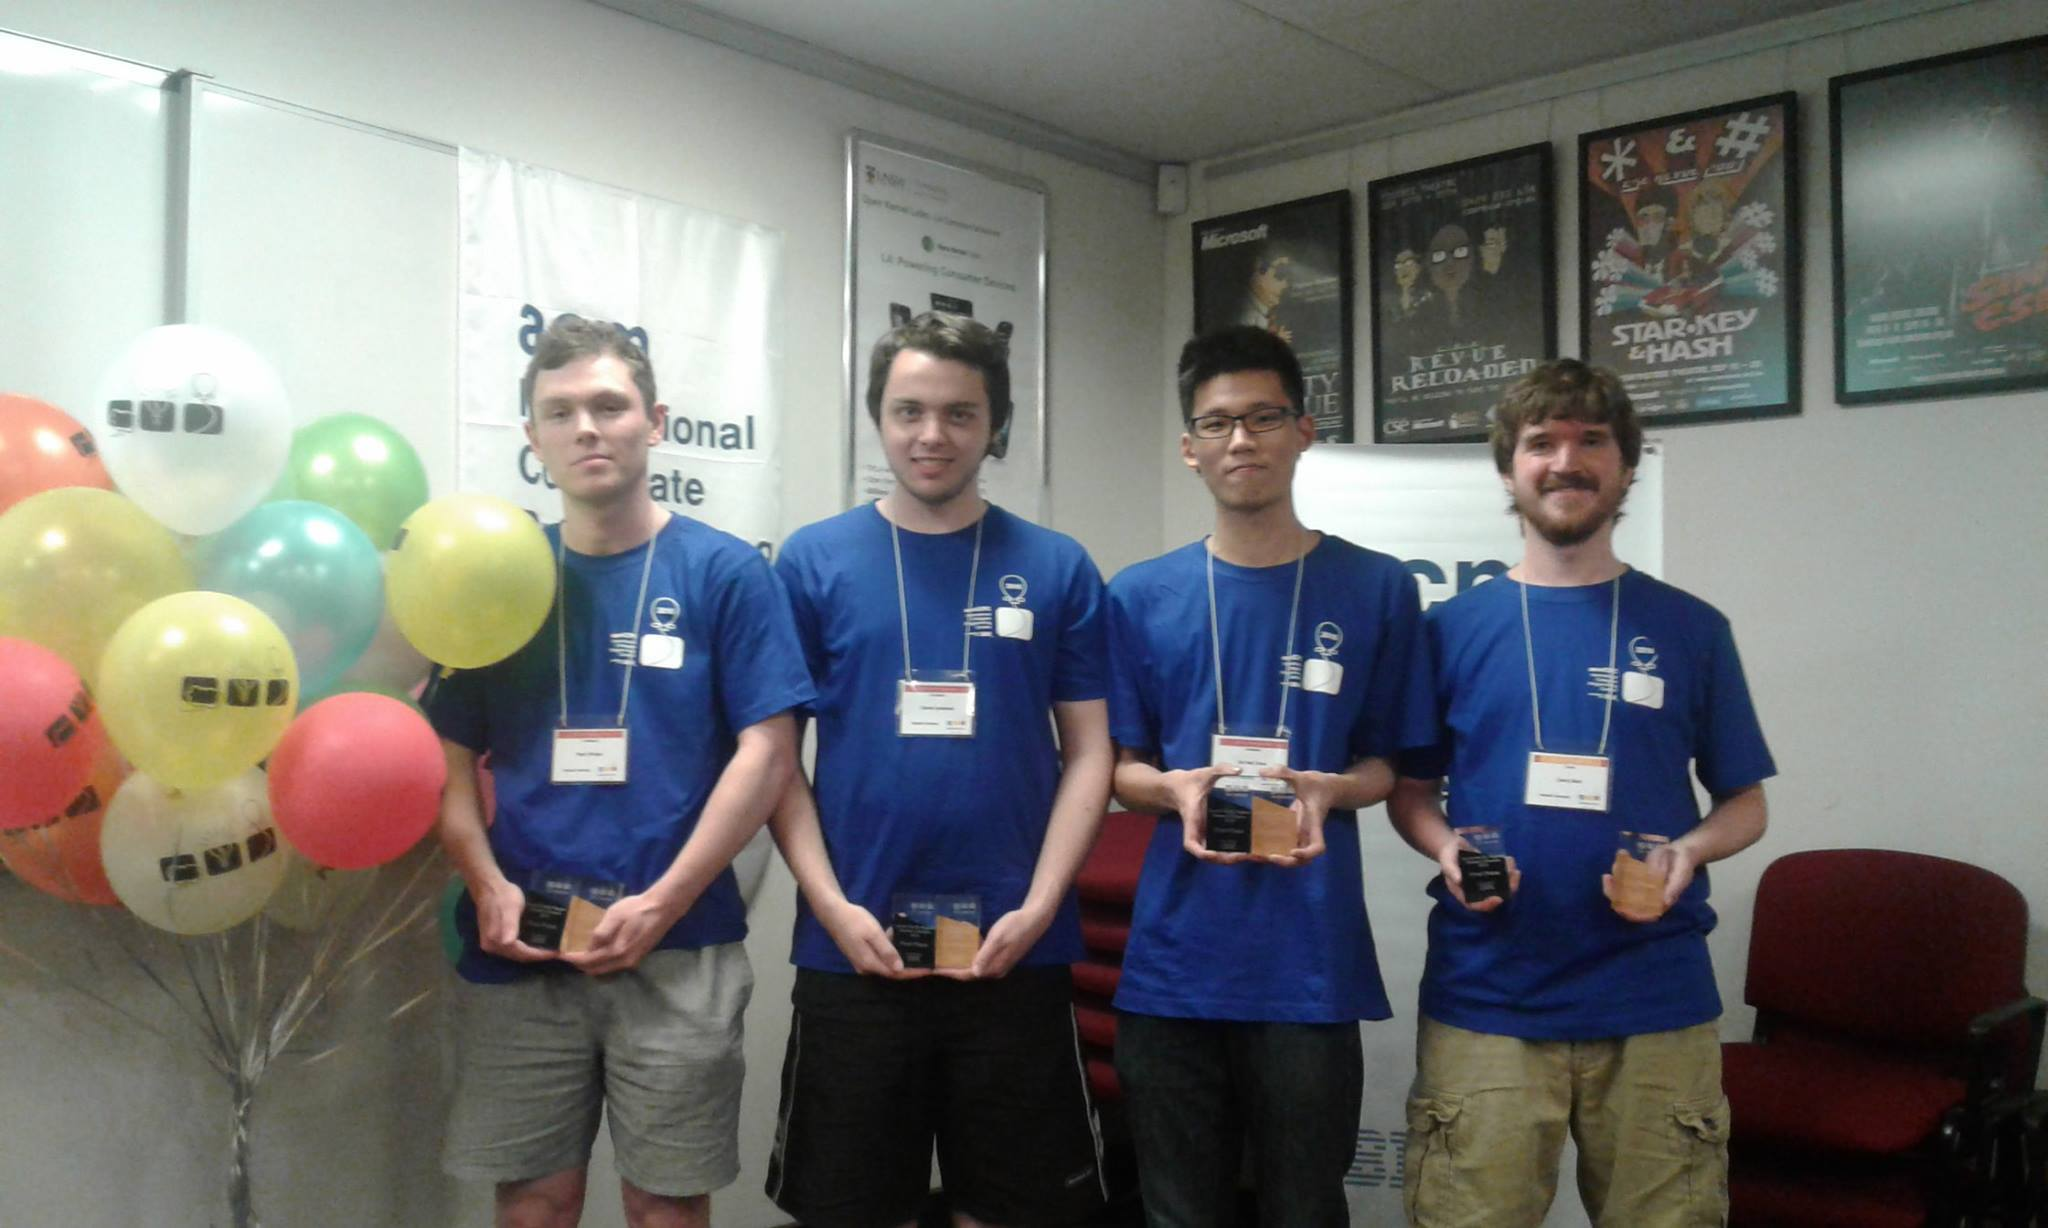
\includegraphics[width=.7\textwidth]{pic/wf2016.jpg}
  \end{figure}
  Get rewarded!
\end{frame}

\begin{frame}{Another Story}
  \begin{figure}
  \centering
  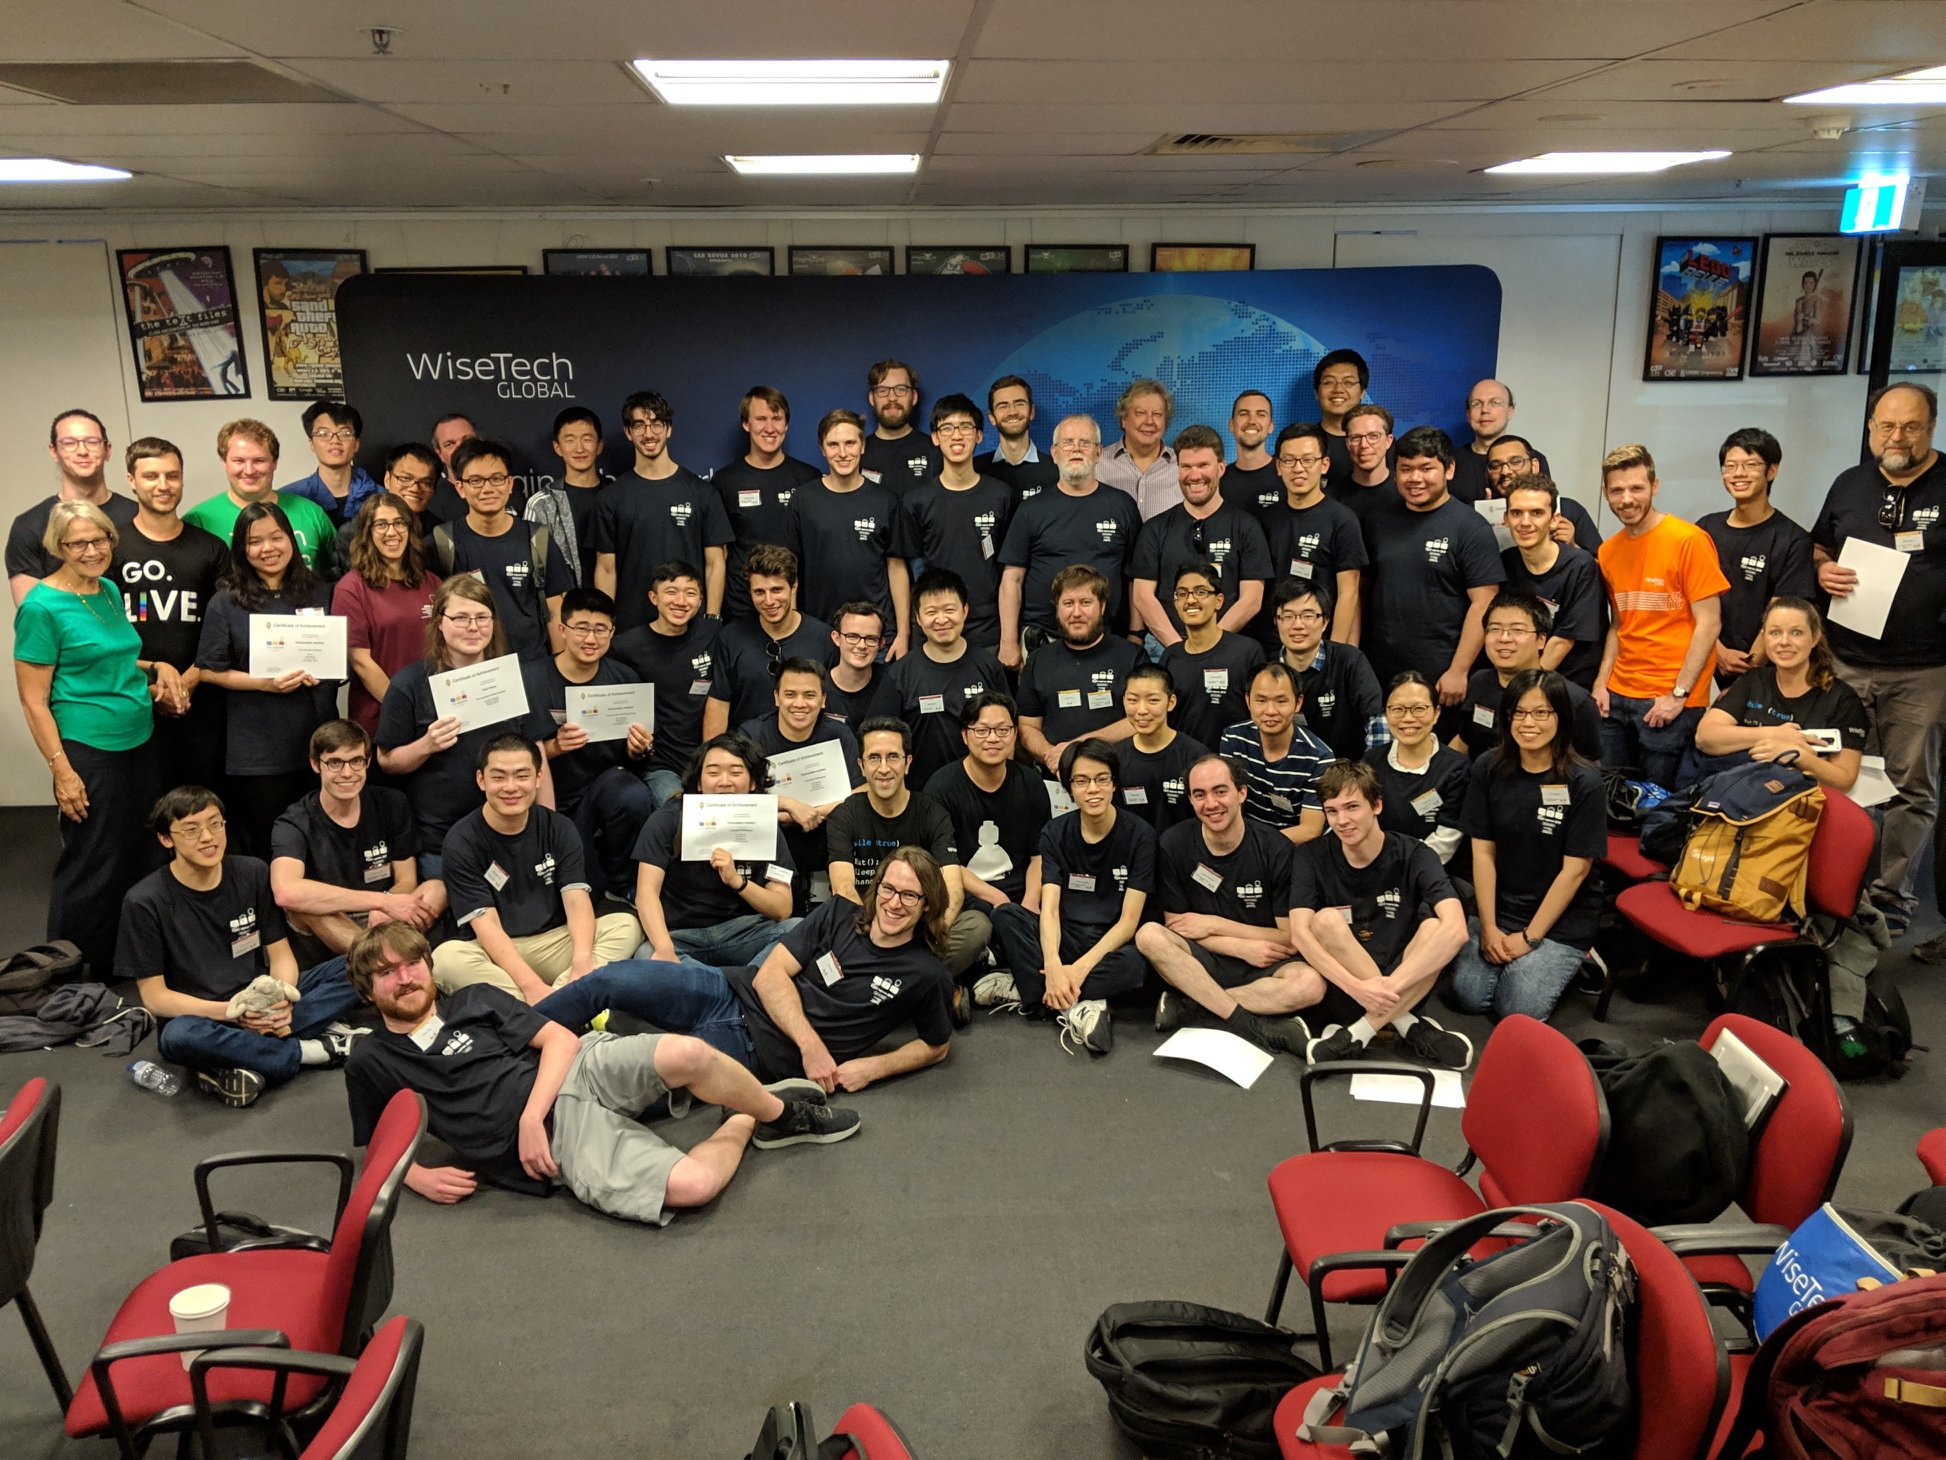
\includegraphics[width=.7\textwidth]{pic/regional-2018.jpg}
  \end{figure}
  Make friends!
\end{frame}

\begin{frame}{Why do we do Competitive Programming?}
  \begin{itemize}
    \item<2-> IT IS FUN!
    \item<3-> Employment
    \item<4-> Academia
  \end{itemize}
\end{frame}

\section{How}
\begin{frame}{How to start?}
  \begin{itemize}
    \item USACO: \small \url {https://train.usaco.org/usacogate}
    \item Codeforces: \small \url {http://codeforces.com}
    \item Atcoder: \small \url {http://atcoder.jp}
    \item Google contests: \small \url {https://codingcompetitions.withgoogle.com}
    \item Facebook Hacker Cup: \small \url {https://www.facebook.com/hackercup/contest}
  \end{itemize}
\end{frame}

\begin{frame}{How to join us?}
  \begin{itemize}
    \item Weekly training on Saturday. \small(12 to 17, Lab 147, Rainforest Walk 14)
    \item Facebook: \small \url {https://www.facebook.com/groups/454114112027992/}
    \item Mailing list: \small \url {https://groups.google.com/forum/\#!forum/monashicpc/join}
  \end{itemize}
\end{frame}

\begin{frame}{What will we do?}
  \begin{itemize}
    \item Monash Collegiate Programming Contest (MCPC) on \textbf{24th August}.
    \item New Zealand Programming Contest (NZPC) on \textbf{7th September}.
    \item International Collegiate Programming Contest (ICPC) Regional Divisional (TBD).
    \item ICPC Regional Final (TBD).
    \item ICPC World Final (TBD, if only...).
  \end{itemize}
\end{frame}

\section{End}
\begin{frame}{End}
    \centering
    \Huge {Join Us! \\ Thank you!}
\end{frame}

% -----------------------------------------------------------------------------
\end{document}
%-----------------------------------------------
